\documentclass{article}
\usepackage{ctex}
\usepackage{graphicx}
\usepackage{amsmath}
\usepackage{indentfirst}
\usepackage{titlesec}
\usepackage{setspace}
\usepackage{subfigure}
\usepackage{caption}
\usepackage{float}
\usepackage{booktabs}
\usepackage{geometry}
\usepackage{multirow}
\usepackage{hyperref}
\hypersetup{
	colorlinks=true,
	linkcolor=blue,
	filecolor=magenta,      
	urlcolor=cyan,
	pdftitle={Overleaf Example},
	pdfpagemode=FullScreen,
}
\geometry{left=1.2cm,right=1.2cm,top=2cm,bottom=2cm}
\title{\songti \zihao{2}\bfseries Nacl晶体原子振荡}
\titleformat*{\section}{\songti\zihao{4}\bfseries}
\titleformat*{\subsection}{\songti\zihao{5}\bfseries}
\renewcommand\thesection{\arabic{section}}
\author{王启骅 PB20020580}
\begin{document}
	\maketitle
	\section{NaCl晶体原子力学分析}
	NaCl晶体的结构如图\ref{fig:1}所示
	\begin{figure}[!h]
	
	\centering
	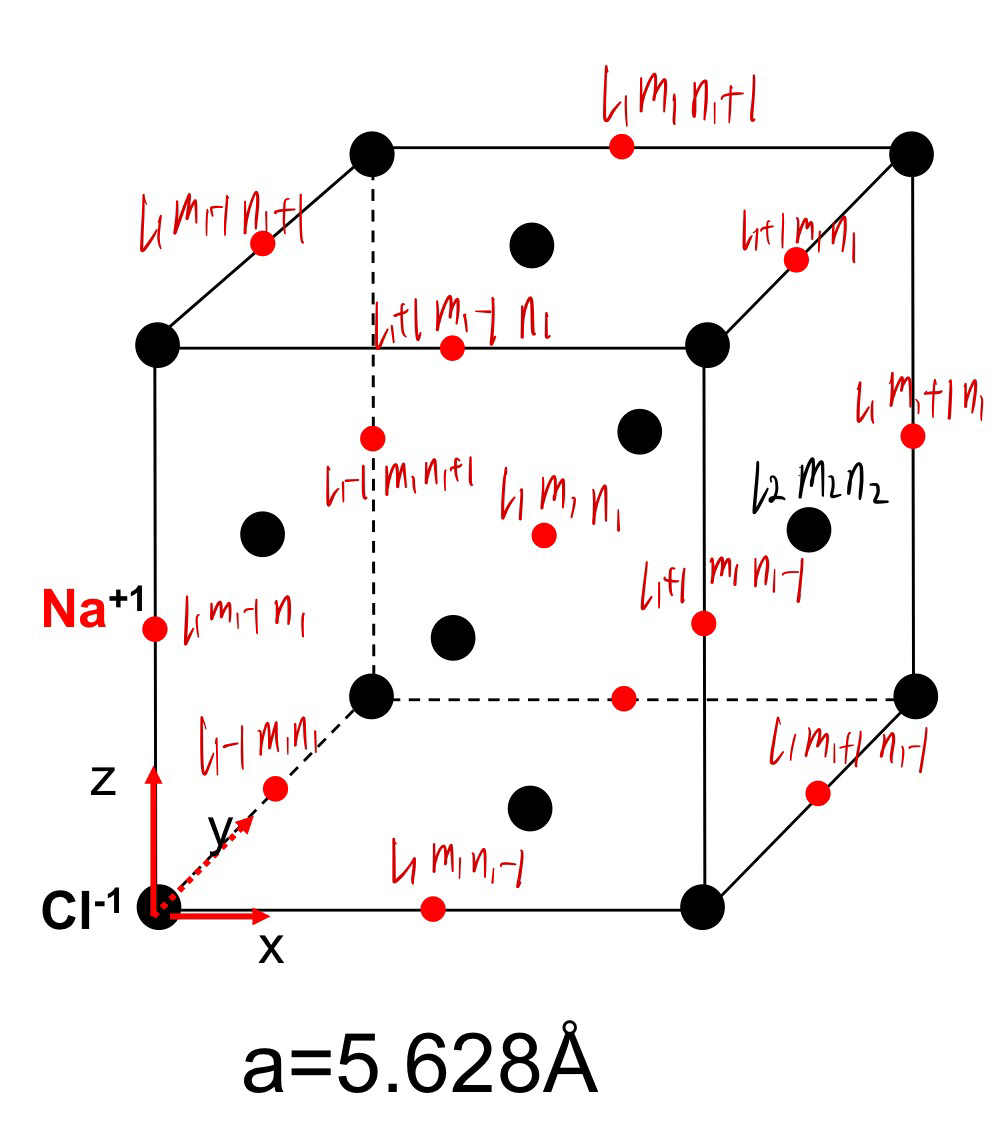
\includegraphics[scale=0.3]{NaCl1}
	\captionsetup{font={small},labelfont=bf}
	\caption{\heiti\zihao{-5}NaCl晶体结构}
	\label{fig:1}%label加最后才可以引用正常
\end{figure}


分别使用l,m,n编号原子的
基矢$ \vec{a_1}=\frac{a}{2}(\hat{x}+\hat{z}),\vec{a_2}=\frac{a}{2}(\hat{x}+\hat{y}),\vec{a_3}=\frac{a}{2}(\hat{y}+\hat{z}) $方向序号。取Na原子与临近x轴正方向的一个Cl原子为原胞,Na原子位于1位置,Cl原子位于2位置。偏移格点的位移用$ u^x,u^y,u^z $表示。假设Na与Cl原子间相互作用力系数为$ \beta $,Na与Na原子之间相互作用系数为$ \beta_1 $,Cl与Cl之间的力相互作用系数为$ \beta_2 $。Na原子质量m,Cl原子质量为M。现在对第$ (l_1,m_1,n_1) $与$ (l_2,m_2,n_2) $的Na原子和Cl原子作为原胞进行受力分析。


首先是Na原子:
\begin{equation}
		\begin{aligned}
			m\ddot{u}^x_{l_1,m_1,n_1}&=-\beta(2u^x_{l_1,m_1,n_1}-u^x_{l_2,m_2,n_2}-u^x_{l_2-1,m_2-1,n_2+1})\\
			&+\frac{\beta_1}{2}\big[(u^x_{(l_1+1)m_1n_1}-u^x_{l_1m_1n_1})+(u^x_{(l_1-1)m_1n_1}-u^x_{l_1m_1n_1})+(u^x_{l_1(m_1+1)n_1}-u^x_{l_1m_1n_1})+(u^x_{l_1(m_1-1)n_1}-u^x_{l_1m_1n_1})\\
			&+(u^x_{(l_1+1)m_1(n_1-1)}-u^x_{l_1m_1n_1})+(u^x_{(l_1-1)m_1(n_1+1)}-u^x_{l_1m_1n_1})+(u^x_{l_1(m_1+1)(n_1-1)}-u^x_{l_1m_1n_1})+(u^x_{l_1(m_1-1)(n_1+1)}-u^x_{l_1m_1n_1})\\
			&+(u^y_{l_1(m_1+1)n_1}-u^y_{l_1m_1n_1})+(u^y_{l_1(m_1-1)n_1}-u^y_{l_1m_1n_1})-(u^y_{(l_1+1)m_1(n_1-1)}-u^y_{l_1m_1n_1})-(u^y_{(l_1-1)m_1(n_1+1)}-u^y_{l_1m_1n_1})\\
			&+(u^z_{(l_1+1)m_1n_1}-u^z_{l_1m_1n_1})+(u^z_{(l_1-1)m_1n_1}-u^z_{l_1m_1n_1})-(u^z_{l_1(m_1+1)(n_1-1)}-u^z_{l_1m_1n_1})-(u^z_{l_1(m_1-1)(n_1+1)}-u^z_{l_1m_1n_1})\big]\\
		\end{aligned}
\end{equation}
\begin{equation}
	\begin{aligned}
		m\ddot{u}^y_{l_1,m_1,n_1}&=-\beta(2u^y_{l_1,m_1,n_1}-u^y_{l_2-1,m_2,n_2+1}-u^y_{l_2,m_2-1,n_2})\\
		&+\frac{\beta_1}{2}\big[(u^y_{l_1m_1(n_1+1)}-u^y_{l_1m_1n_1})+(u^y_{l_1m_1(n_1-1)}-u^y_{l_1m_1n_1})+(u^y_{l_1(m_1+1)n_1}-u^y_{l_1m_1n_1})+(u^y_{l_1(m_1-1)n_1}-u^y_{l_1m_1n_1})\\
		&+(u^y_{(l_1+1)m_1(n_1-1)}-u^y_{l_1m_1n_1})+(u^y_{(l_1-1)m_1(n_1+1)}-u^y_{l_1m_1n_1})+(u^y_{(l_1-1)(m_1+1)n_1}-u^y_{l_1m_1n_1})+(u^y_{(l_1+1)(m_1-1)n_1}-u^y_{l_1m_1n_1})\\
		&+(u^x_{l_1(m_1+1)n_1}-u^x_{l_1m_1n_1})+(u^x_{l_1(m_1-1)n_1}-u^x_{l_1m_1n_1})-(u^x_{(l_1+1)m_1(n_1-1)}-u^x_{l_1m_1n_1})-(u^x_{(l_1-1)m_1(n_1+1)}-u^x_{l_1m_1n_1})\\
		&+(u^z_{l_1m_1(n_1+1)}-u^z_{l_1m_1n_1})+(u^z_{l_1m_1(n_1-1)}-u^z_{l_1m_1n_1})-(u^z_{(l_1-1)(m_1+1)n_1}-u^z_{l_1m_1n_1})-(u^z_{(l_1+1)(m_1-1)n_1}-u^z_{l_1m_1n_1})\big]\\
	\end{aligned}
\end{equation}
\begin{equation}
	\begin{aligned}
		m\ddot{u}^z_{l_1,m_1,n_1}&=-\beta(2u^z_{l_1,m_1,n_1}-u^z_{l_2,m_2-1,n_2+1}-u^z_{l_2-1,m_2,n_2})\\
		&+\frac{\beta_1}{2}\big[(u^z_{l_1m_1(n_1+1)}-u^z_{l_1m_1n_1})+(u^z_{l_1m_1(n_1-1)}-u^z_{l_1m_1n_1})+(u^z_{(l_1+1)m_1n_1}-u^z_{l_1m_1n_1})+(u^z_{(l_1-1)m_1n_1}-u^y_{l_1m_1n_1})\\
		&+(u^z_{l_1(m_1+1)(n_1-1)}-u^z_{l_1m_1n_1})+(u^z_{l_1(m_1-1)(n_1+1)}-u^z_{l_1m_1n_1})+(u^z_{(l_1-1)(m_1+1)n_1}-u^z_{l_1m_1n_1})+(u^z_{(l_1+1)(m_1-1)n_1}-u^z_{l_1m_1n_1})\\
		&+(u^x_{(l_1+1)m_1n_1}-u^x_{l_1m_1n_1})+(u^x_{(l_1-1)m_1n_1}-u^x_{l_1m_1n_1})-(u^x_{l_1(m_1-1)(n_1+1)}-u^x_{l_1m_1n_1})-(u^x_{l_1(m_1+1)(n_1-1)}-u^x_{l_1m_1n_1})\\
		&+(u^y_{l_1m_1(n_1+1)}-u^y_{l_1m_1n_1})+(u^y_{l_1m_1(n_1-1)}-u^y_{l_1m_1n_1})-(u^y_{(l_1-1)(m_1+1)n_1}-u^y_{l_1m_1n_1})-(u^y_{(l_1+1)(m_1-1)n_1}-u^y_{l_1m_1n_1})\big]\\
	\end{aligned}
\end{equation}


类似对于Cl原子
\begin{equation}
	\begin{aligned}
		M\ddot{u}^x_{l_2,m_2,n_2}&=-\beta(2u^x_{l_2,m_2,n_2}-u^x_{l_1,m_1,n_1}-u^x_{l_1+1,m_1+1,n_1-1})\\
		&+\frac{\beta_2}{2}\big[(u^x_{(l_2+1)m_2n_2}-u^x_{l_2m_2n_2})+(u^x_{(l_2-1)m_2n_2}-u^x_{l_2m_2n_2})+(u^x_{l_2(m_2+1)n_2}-u^x_{l_2m_2n_2})+(u^x_{l_2(m_2-1)n_2}-u^x_{l_2m_2n_2})\\
		&+(u^x_{(l_2+1)m_2(n_2-1)}-u^x_{l_2m_2n_2})+(u^x_{(l_2-1)m_2(n_2+1)}-u^x_{l_2m_2n_2})+(u^x_{l_2(m_2+1)(n_2-1)}-u^x_{l_2m_2n_2})+(u^x_{l_2(m_2-1)(n_2+1)}-u^x_{l_2m_2n_2})\\
		&+(u^y_{l_2(m_2+1)n_2}-u^y_{l_2m_2n_2})+(u^y_{l_2(m_2-1)n_2}-u^y_{l_2m_2n_2})-(u^y_{(l_2+1)m_2(n_2-1)}-u^y_{l_2m_2n_2})-(u^y_{(l_2-1)m_2(n_2+1)}-u^y_{l_2m_2n_2})\\
		&+(u^z_{(l_2+1)m_2n_2}-u^z_{l_2m_2n_2})+(u^z_{(l_2-1)m_2n_2}-u^z_{l_2m_2n_2})-(u^z_{l_2(m_2+1)(n_2-1)}-u^z_{l_2m_2n_2})-(u^z_{l_2(m_2-1)(n_2+1)}-u^z_{l_2m_2n_2})\big]\\
	\end{aligned}
\end{equation}
\begin{equation}
	\begin{aligned}
		M\ddot{u}^y_{l_2,m_2,n_2}&=-\beta(2u^y_{l_2,m_2,n_2}-u^y_{l_1,m_1+1,n_1}-u^y_{l_1+1,m_1,n_1-1})\\
		&+\frac{\beta_2}{2}\big[(u^y_{l_2m_2(n_2+1)}-u^y_{l_2m_2n_2})+(u^y_{l_2m_2(n_2-1)}-u^y_{l_2m_2n_2})+(u^y_{l_2(m_2+1)n_2}-u^y_{l_2m_2n_2})+(u^y_{l_2(m_2-1)n_2}-u^y_{l_2m_2n_2})\\
		&+(u^y_{(l_2+1)m_2(n_2-1)}-u^y_{l_2m_2n_2})+(u^y_{(l_2-1)m_2(n_2+1)}-u^y_{l_2m_2n_2})+(u^y_{(l_2-1)(m_2+1)n_2}-u^y_{l_2m_2n_2})+(u^y_{(l_2+1)(m_2-1)n_2}-u^y_{l_2m_2n_2})\\
		&+(u^x_{l_2(m_2+1)n_2}-u^x_{l_2m_2n_2})+(u^x_{l_2(m_2-1)n_2}-u^x_{l_2m_2n_2})-(u^x_{(l_2+1)m_2(n_2-1)}-u^x_{l_2m_2n_2})-(u^x_{(l_2-1)m_2(n_2+1)}-u^x_{l_2m_2n_2})\\
		&+(u^z_{l_2m_2(n_2+1)}-u^z_{l_2m_2n_2})+(u^z_{l_2m_2(n_2-1)}-u^z_{l_2m_2n_2})-(u^z_{(l_2-1)(m_2+1)n_2}-u^z_{l_2m_2n_2})-(u^z_{(l_2+1)(m_2-1)n_2}-u^z_{l_2m_2n_2})\big]\\
	\end{aligned}
\end{equation}
\begin{equation}
	\begin{aligned}
		M\ddot{u}^z_{l_2,m_2,n_2}&=-\beta(2u^z_{l_2,m_2,n_2}-u^z_{l_1+1,m_1,n_1}-u^z_{l_1,m_1+1,n_1-1})\\
		&+\frac{\beta_2}{2}\big[(u^z_{l_2m_2(n_2+1)}-u^z_{l_2m_2n_2})+(u^z_{l_2m_2(n_2-1)}-u^z_{l_2m_2n_2})+(u^z_{(l_2+1)m_2n_2}-u^z_{l_2m_2n_2})+(u^z_{(l_2-1)m_2n_2}-u^y_{l_2m_2n_2})\\
		&+(u^z_{l_2(m_2+1)(n_2-1)}-u^z_{l_2m_2n_2})+(u^z_{l_2(m_2-1)(n_2+1)}-u^z_{l_2m_2n_2})+(u^z_{(l_2-1)(m_2+1)n_2}-u^z_{l_2m_2n_2})+(u^z_{(l_2+1)(m_2-1)n_2}-u^z_{l_2m_2n_2})\\
		&+(u^x_{(l_2+1)m_2n_2}-u^x_{l_2m_2n_2})+(u^x_{(l_2-1)m_2n_2}-u^x_{l_2m_2n_2})-(u^x_{l_2(m_2-1)(n_2+1)}-u^x_{l_2m_2n_2})-(u^x_{l_2(m_2+1)(n_2-1)}-u^x_{l_2m_2n_2})\\
		&+(u^y_{l_2m_2(n_2+1)}-u^y_{l_2m_2n_2})+(u^y_{l_2m_2(n_2-1)}-u^y_{l_2m_2n_2})-(u^y_{(l_2-1)(m_2+1)n_2}-u^y_{l_2m_2n_2})-(u^y_{(l_2+1)(m_2-1)n_2}-u^y_{l_2m_2n_2})\big]\\
	\end{aligned}
\end{equation}


可以得到方程解的形式为
\begin{equation}
	\vec{u}_{l_1m_1n_1}=\vec{A}\exp i[wt-\vec{k}\cdot\vec{a}_1l_1-\vec{k}\cdot\vec{a}_2m_1-\vec{k}\cdot\vec{a}_3n_1]
\end{equation}
\begin{equation}
	\vec{u}_{l_2m_2n_2}=\vec{B}\exp i[wt-\vec{k}\cdot\vec{a}_1l_2-\vec{k}\cdot\vec{a}_2m_2-\vec{k}\cdot\vec{a}_3n_2]
\end{equation}


根据Na原子与Cl原子位置关系可得$ (l_2,m_2,n_2)=(l_1+\frac{1}{2},m_1+\frac{1}{2},n_1-\frac{1}{2}) $。
\begin{equation}
	\vec{u}_{l_1m_1n_1}=\vec{A}\exp i[wt-k_xa\frac{l_1+m_1}{2}-k_ya\frac{m_1+n_1}{2}-k_za\frac{l_1+n_1}{2}]
	\label{eq9}
\end{equation}
\begin{equation}
	\vec{u}_{l_2m_2n_2}=\vec{B}\exp i[wt-k_xa\frac{l_1+m_1+1}{2}-k_ya\frac{m_1+n_1}{2}-k_za\frac{l_1+n_1}{2}]
	\label{eq10}
\end{equation}


将解反代回方程(\ref{eq9})(\ref{eq10}) 可以得
	\begin{equation}
		\begin{aligned}
			0&=\{\beta_1[4-\cos\frac{a}{2}(k_x+k_z)-\cos\frac{a}{2}(k_x-k_z)-\cos\frac{a}{2}(k_x+k_y)-\cos\frac{a}{2}(k_x-k_y)]+2\beta-mw^2\}A_x\\
			&+\beta_1[\cos\frac{a}{2}(k_x-k_y)-\cos\frac{a}{2}(k_x+k_y)]A_y+\beta_1[\cos\frac{a}{2}(k_x-k_z)-\cos\frac{a}{2}(k_x+k_z)]A_z-2\beta\cos(\frac{a}{2}k_x)B_x
		\end{aligned}
	\end{equation}
	\begin{equation}
	\begin{aligned}
		0&=\{\beta_1[4-\cos\frac{a}{2}(k_y+k_z)-\cos\frac{a}{2}(k_y-k_z)-\cos\frac{a}{2}(k_x+k_y)-\cos\frac{a}{2}(k_x-k_y)]+2\beta-mw^2\}A_y\\
		&+\beta_1[\cos\frac{a}{2}(k_x-k_y)-\cos\frac{a}{2}(k_x+k_y)]A_x+\beta_1[\cos\frac{a}{2}(k_y-k_z)-\cos\frac{a}{2}(k_y+k_z)]A_z-2\beta\cos(\frac{a}{2}k_y)B_y
	\end{aligned}
\end{equation}
	\begin{equation}
	\begin{aligned}
		0&=\{\beta_1[4-\cos\frac{a}{2}(k_x+k_z)-\cos\frac{a}{2}(k_x-k_z)-\cos\frac{a}{2}(k_z+k_y)-\cos\frac{a}{2}(k_z-k_y)]+2\beta-mw^2\}A_z\\
		&+\beta_1[\cos\frac{a}{2}(k_x-k_z)-\cos\frac{a}{2}(k_x+k_z)]A_x+\beta_1[\cos\frac{a}{2}(k_y-k_z)-\cos\frac{a}{2}(k_y+k_z)]A_y-2\beta\cos(\frac{a}{2}k_z)B_z
	\end{aligned}
\end{equation}
	\begin{equation}
	\begin{aligned}
		0&=\{\beta_2[4-\cos\frac{a}{2}(k_x+k_z)-\cos\frac{a}{2}(k_x-k_z)-\cos\frac{a}{2}(k_x+k_y)-\cos\frac{a}{2}(k_x-k_y)]+2\beta-Mw^2\}B_x\\
		&+\beta_2[\cos\frac{a}{2}(k_x-k_y)-\cos\frac{a}{2}(k_x+k_y)]B_y+\beta_2[\cos\frac{a}{2}(k_x-k_z)-\cos\frac{a}{2}(k_x+k_z)]B_z-2\beta\cos(\frac{a}{2}k_x)A_x
	\end{aligned}
\end{equation}
	\begin{equation}
	\begin{aligned}
		0&=\{\beta_2[4-\cos\frac{a}{2}(k_y+k_z)-\cos\frac{a}{2}(k_y-k_z)-\cos\frac{a}{2}(k_x+k_y)-\cos\frac{a}{2}(k_x-k_y)]+2\beta-Mw^2\}B_y\\
		&+\beta_2[\cos\frac{a}{2}(k_x-k_y)-\cos\frac{a}{2}(k_x+k_y)]B_x+\beta_2[\cos\frac{a}{2}(k_y-k_z)-\cos\frac{a}{2}(k_y+k_z)]B_z-2\beta\cos(\frac{a}{2}k_y)A_y
	\end{aligned}
\end{equation}
	\begin{equation}
	\begin{aligned}
		0&=\{\beta_2[4-\cos\frac{a}{2}(k_x+k_z)-\cos\frac{a}{2}(k_x-k_z)-\cos\frac{a}{2}(k_z+k_y)-\cos\frac{a}{2}(k_z-k_y)]+2\beta-Mw^2\}B_z\\
		&+\beta_2[\cos\frac{a}{2}(k_z-k_y)-\cos\frac{a}{2}(k_z+k_y)]B_y+\beta_2[\cos\frac{a}{2}(k_x-k_z)-\cos\frac{a}{2}(k_x+k_z)]B_x-2\beta\cos(\frac{a}{2}k_z)A_z
	\end{aligned}
\end{equation}


计算矩阵行列式得到w的12次方程,为了简化计算,我们取波沿x方向传播,即$ k_x=k,k_y=k_z=0 $,可以得到w的2个3重正根如下
\begin{equation}
	\begin{aligned}
w_1(k)&=w_2(k)=w_3(k)=\bigg(\frac{\beta}{m}+\frac{\beta}{M}+\frac{\beta_1}{m}-\frac{\cos(\frac{ak}{2})\beta_1}{m}+\frac{\beta_2}{M}-\frac{\cos(\frac{ak}{2})\beta_2}{M}\\
	&-\frac{1}{2mM}\big( (-2m\beta-2M\beta-2M\beta_1+2M\cos(\frac{ak}{2})\beta_1-2m\beta_2+2m\cos(\frac{ak}{2})\beta_2)^2\\
	&-4mM(4\beta\beta_1-4\beta\cos(\frac{ak}{2})\beta_1+4\beta\beta_2-4\beta\cos(\frac{ak}{2})\beta_2+6\beta_1\beta_2-8\cos(\frac{ak}{2})\beta_1\beta_2+2\cos(ak)\beta_1\beta_2) \big)^{\frac{1}{2}}\bigg) ^{\frac{1}{2}}
 	\end{aligned}
\end{equation}
\begin{equation}
	\begin{aligned}
		&w_4(k)=w_5(k)=w_6(k)=\bigg(\frac{\beta}{m}+\frac{\beta}{M}+\frac{2\beta_1}{m}-\frac{2\cos(\frac{ak}{2})\beta_1}{m}+\frac{2\beta_2}{M}-\frac{2\cos(\frac{ak}{2})\beta_2}{M}\\
		&-\frac{1}{2mM}\big( (-2m\beta-2M\beta-4M\beta_1+4M\cos(\frac{ak}{2})\beta_1-4m\beta_2+4m\cos(\frac{ak}{2})\beta_2)^2\\
		&-4mM(2\beta^2-2\beta^2\cos(ak)+8\beta\beta_1-8\beta\cos(\frac{ak}{2})\beta_1+8\beta\beta_2-8\beta\cos(\frac{ak}{2})\beta_2+24\beta_1\beta_2-32\cos(\frac{ak}{2})\beta_1\beta_2+8\cos(ak)\beta_1\beta_2) \big)^{\frac{1}{2}}\bigg) ^{\frac{1}{2}}
	\end{aligned}
\end{equation}


计算当$ k\rightarrow 0 $可得$ w_1,w_2,w_3\rightarrow0 $为声学支,$ w_4,w_5,w_6\rightarrow \sqrt{\frac{2\beta}{M}+\frac{2\beta}{m}} $为光学支。由于我们主要关心曲线的趋势,可将相关的参数取为$\beta =\beta_1 = \beta_2,M=35.5/23*m $,作图如图\ref{fig:2}
	\begin{figure}[!h]
	
	\centering
	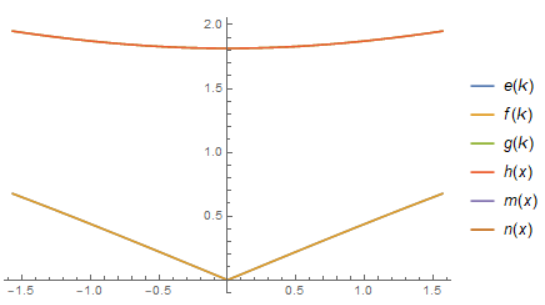
\includegraphics[scale=0.85]{mode}
	\captionsetup{font={small},labelfont=bf}
	\caption{\heiti\zihao{-5}NaCl晶体色散关系}
	\label{fig:2}%label加最后才可以引用正常
\end{figure}
其中横坐标为$ ak $,纵坐标为$ \sqrt{\frac{m}{\beta}}w $


这里另解了$ k_x=k_y=k_z=\frac{k}{\sqrt{3}}$的情况,如图\ref{fig:3},存在3个相同的声学支,3个光学支中1个2重根与1个单根。
	\begin{figure}[!h]
	
	\centering
	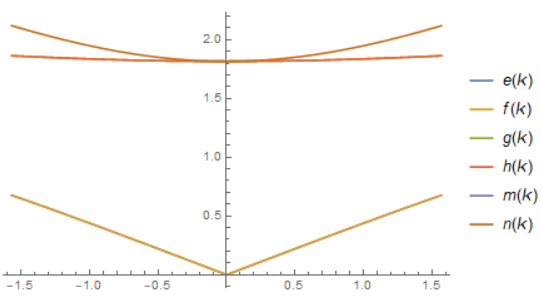
\includegraphics[scale=0.9]{mode_2}
	\captionsetup{font={small},labelfont=bf}
	\caption{\heiti\zihao{-5}NaCl晶体色散关系}
	\label{fig:3}%label加最后才可以引用正常
\end{figure}
\section{结果讨论}
由此可见确实都有3个声学支。本次计算中由于取了特殊沿对称轴方向的波矢,导致根存在一定的简并,如果选取更多的较为一般的波矢方向,则可得到更多分立的解。
\end{document}